% !TEX root = template.tex

\section{Introduction}

Here goes the introduction. We also cite the nice book by \citet{Pinedo:2012}.
This might be a book with interesting topics, but concurrent time-stamping has also been addressed before~\cite{Dolev97}.
In this work, \citet{Dolev97} presented the first bounded implementation of a concurrent time-stamp system.

\section{Scheduling Algorithm}

\citet*{Chen2017} view a data analytic \emph{job} simply as a number of \emph{tasks} that comprise it. These tasks are further separated into consecutive \emph{stages}, where the future stages depend on the results of the past stages. In other words, the tasks from a single stage must wait for the tasks from all the previous stages to complete. On the contrary, within a single stage the tasks are \emph{independent} of each other and therefore could be executed in parallel.

\citet{Chen2017} further describe a geographically distributed datacenter as a group of independent datacenters connected by a network. Each single datacenter from this group consists of a number of available \emph{computing slots}. Furthermore, the network that connects the pairs of datacenters is expected to have significantly \emph{lower bandwidth} than the local network of each individual datacenter. This means that transferring large amounts of data between different datacenters takes a lot of time. Finally, in order to execute a task, it must be provided with a computing slot and the necessary input data. The input data for every task is also hosted by some datacenter(s). If it so happens that a task is assigned to a datacenter that does not hold the entire input data for that task, the missing parts will have to be transferred across the inter-datacenter network.

\subsection{Formal Definitions}

\citet*{Chen2017} define \(\mathcal{D} = \left\{1, 2, \dots, J\right\}\) to be the set whose elements are individual datacenters and the entire set itself represents one large geographically distributed datacenter. Each individual datacenter \(i\) has a limited number of computing slots denoted by \(a_i\). Furthermore, the set of analytic jobs is defined as \(\mathcal{K} = \left\{1, 2, \dots, K\right\}\). Each of the jobs \(k\) consists of a single stage which itself is a set of independent tasks \(\mathcal{T}_k=\left\{1, 2, \dots, n_k\right\}\).

In the proposed theoretical model the time it takes to complete a job is the \emph{longest} time one if its independent tasks takes to complete. In turn, the completion time of a task is the sum \(e^{k}_{i, j} + c^{k}_{i, j}\), where the first summand is the \emph{execution time} and the second --- \emph{network transfer time}. For both of them, index \(i\) is the analytic job, index \(k\) is the task from that job and index \(j\) is the index of the datacenter to which the task is assigned. The execution time for any possible assignment is assumed to be known in advance. The network transfer time, on the other hand, is calculated in a slightly more complicated fashion. Task \(k\) of job \(i\) requires input data that is stored by a set of individual datacenters \(S^k_i\). More specifically, for each datacenter \(s\in S^k_i\) the volume of input data is \(d^{k, s}_i\). Assuming \(s\neq j\), the bandwidth between these two datacenters is \(b_{s, j}\). Then the following formula computes network transfer time:

\begin{IEEEeqnarray*}{lCl}
  c^k_{i, j} &=&\left\{ \,
  \begin{IEEEeqnarraybox}[][c]{l?s}
    \IEEEstrut
    0, &  when \(S^k_i = \left\{j\right\}\)\\
    \max_{s\in S^k_i, s\neq j}\left(\frac{d^{k, s}_i}{b_{s,j}}\right) & otherwise
    \IEEEstrut
  \end{IEEEeqnarraybox}
  \right. \\
\end{IEEEeqnarray*}



\subsection{Optimization Problem}
\subsection{Proposed Scheduling Algorithm}

%% Table~\ref{tab:related_algorithms} shows a summary of related algorithms.

%% \begin{table}[h]
%% \centering
%% \captionabove{Related algorithms and their complexity.}
%% \label{tab:related_algorithms}
%% \begin{tabular}{ll}
%% \toprule 
%% algorithm & complexity \\
%% \midrule
%% algorithm Y & $\mathcal{O}(n)$ \\
%% algorithm Z & $\mathcal{O}(n \log{n} )$ \\
%% \bottomrule
%% \end{tabular}
%% \end{table}

\section{Evaluation of the Scheduling Algorithm}


%% \subsection{Evaluating the Running Time of Algorithm X}

%% The run-time of our algorithm is shown in Figure~\ref{fig:runtime}.
%% We can observe that the run-time of our algorithm increases linearly with the message size.
%% Since we target a system with a run-time of less than \SI{10}{\second}, the maximum message size should be \SI{128}{\byte}.

%% \begin{figure}[h]
%% \centering
%% 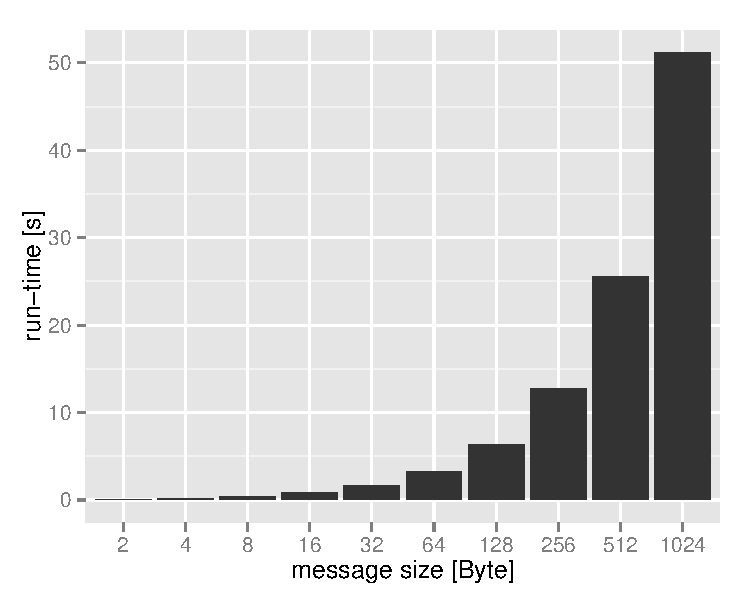
\includegraphics[width=.5\linewidth]{figures/runtime}
%% \caption{Run-time of algorithm X on machine Y.}
%% \label{fig:runtime}
%% \end{figure}

%% \subsection{Evaluating the Space Requirements of Algorithm X}

%% Now, we investigate the space requirements of the algorithms listed in Table~\ref{tab:related_algorithms}.


\section{Summary}
We summary the contribution of the papers and this seminar paper.
